\begin{figure}[h]
	\centering
	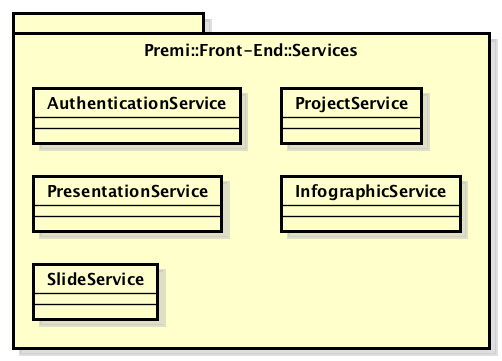
\includegraphics[width=0.7\linewidth]{img/premi_front_end_services}
	\caption[Premi::Front-End::Services]{Premi::Front-End::Services}
\end{figure}
Il package gestisce i services del front-end. Comunica con il model e i controller per creare le funzioni comuni ad essi e richiamarle. È inoltre il responsabile delle chiamate alle API REST del back-end per salvare e caricare i dati dal database.

\subsubsection{AuthenticationService}
	\begin{figure}[h]
		\centering
		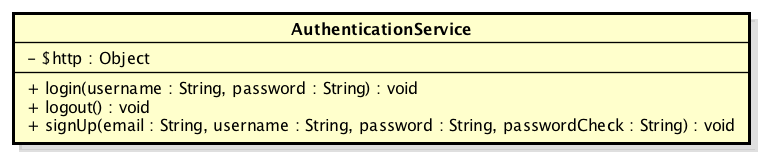
\includegraphics[width=0.6\linewidth]{img/premi_front_end_services_authenticationservice}
		\caption[Premi::Front-End::Services::AuthenticationService]{Premi::Front-End::Services::AuthenticationService}
	\end{figure}
	
	\paragraph{Descrizione}
	Questa classe si occupa di gestire il processo di autenticazione e registrazione di un utente.
	
	\paragraph{Utilizzo}
	Viene utilizzata per fornire ai controllers le funzionalità di autenticazione e di registrazione di un utente.
	
	\paragraph{Relazioni con le altre classi}
	\begin{itemize}
		\item \textbf{\textit{IN} Login Controller}
		Classe che gestisce le operazioni e la logica applicativa riguardante il login e la rispettiva pagina;
		\item \textbf{\textit{IN} SignUp Controller}
		Classe che gestisce le operazioni e la logica applicativa riguardante la registrazione e la rispettiva pagina;
		\item \textbf{\textit{IN} ProjectsController}
		Classe che gestisce le operazioni e la logica applicativa riguardante la pagina dell'utente e dei suoi progetti.
	\end{itemize}
	
	\paragraph{Attributi}
	\begin{itemize}
		\item \textbf{+ \$http: Object}:\\
		Campo dati contenente un riferimento al servizio \textit{\$http} creato da Angular per facilitare la comunicazione tramite protocollo HTTP;
	\end{itemize}
	
	\paragraph{Metodi}
	\begin{itemize}
		\item \textbf{+ login(username: String, password: String)}:\\
		Metodo che richiede al back-end l'autenticazione dell'utente tramite i parametri passati alla funzione;
		\item \textbf{+ logout()}:\\
		Metodo che richiede al back-end la de-autenticazione dell'utente dal sistema;
		\item \textbf{+ signUp(email: String, username: String, password: String, passwordCheck: String)}:\\
		Metodo che richiede al back-end di registrare un nuovo utente con i parametri passati alla funzione. Prima di richiamare l'apposita funzione del back-end controlla che le due password coincidano.
	\end{itemize}
	
	d
\subsubsection{InfographicsService}
	\begin{figure}[h]
		\centering
		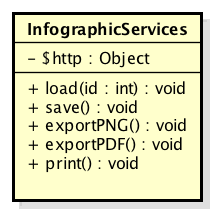
\includegraphics[width=0.4\linewidth]{img/premi_front_end_services_infographicservice}
		\caption[Premi::Front-End::Services::InfographicService]{Premi::Front-End::Services::InfographicService}
	\end{figure}
	
	\paragraph{Descrizione}
	Questa classe si occupa di gestire i processi di visualizzazione e creazione delle infografiche.
	
	\paragraph{Utilizzo}
	Viene utilizzata per fornire ai controllers le funzionalità di interagire con le infografiche.
	
	\paragraph{Relazioni con le altre classi}
	\begin{itemize}
		\item \textbf{\textit{IN} InfographicEditorController}
		Classe che gestisce le operazioni e la logica applicativa riguardante le infografiche;
		\item \textbf{\textit{IN} ProjectController}
		Classe che gestisce le operazioni e la logica applicativa riguardante il progetto di un utente.
	\end{itemize}
	
	\paragraph{Attributi}
	\begin{itemize}
		\item \textbf{+ \$http: Object}:\\
		Campo dati contenente un riferimento al servizio \textit{\$http} creato da Angular per facilitare la comunicazione tramite protocollo HTTP;
	\end{itemize}
	
	\paragraph{Metodi}
	\begin{itemize}
		\item \textbf{+ load(id: int)}:\\
		Metodo che richiede al back-end il caricamento dell'infografica con id quello passato per parametro;
		\item \textbf{+ save()}:\\
		Metodo che richiede al back-end il salvataggio dell'infografica corrente;
		\item \textbf{+ exportPNG()}:\\
		Metodo che esporta l'infografica in un file immagine con estensione .png;
		\item \textbf{+ exportPDF()}:\\
		Metodo che esporta l'infografica in un file con estensione .png;
		\item \textbf{+ print()}:\\
		Metodo che permette di stampare l'infografica.
	\end{itemize}
	
	
\subsubsection{ProjectService}
	\begin{figure}[h]
		\centering
		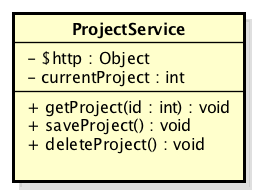
\includegraphics[width=0.4\linewidth]{img/premi_front_end_services_projectservice}
		\caption[Premi::Front-End::Services::ProjectService]{Premi::Front-End::Services::ProjectService}
	\end{figure}
	
	\paragraph{Descrizione}
	Questa classe si occupa di gestire i processi di gestione relativi ai progetti.
	
	\paragraph{Utilizzo}
	Viene utilizzata per fornire ai controllers le funzionalità di interagire con i progetti.
	
	\paragraph{Relazioni con le altre classi}
	\begin{itemize}
		\item \textbf{\textit{IN} ProjectsController}
		Classe che gestisce le operazioni e la logica applicativa riguardante la pagina dell'utente e dei suoi progetti;
		\item \textbf{\textit{IN} ProjectController}
		Classe che gestisce le operazioni e la logica applicativa riguardante il progetto di un utente;
		\item \textbf{\textit{OUT} PresentationEditorController}
		Classe che gestisce le operazioni e la logica applicativa riguardante la modifica di una presentazione;
		\item \textbf{\textit{OUT} InfographicEditorController}
		Classe che gestisce le operazioni e la logica applicativa riguardante la modifica e la gestione di un'infografica.
	\end{itemize}
	
	\paragraph{Attributi}
	\begin{itemize}
		\item \textbf{+ \$http: Object}:\\
		Campo dati contenente un riferimento al servizio \textit{\$http} creato da Angular per facilitare la comunicazione tramite protocollo HTTP;
		\item \textbf{currentProject: int};\\
		Campo dati per contenere l'id del progetto corrente attualmente aperto.
	\end{itemize}
	
	\paragraph{Metodi}
	\begin{itemize}
		\item \textbf{+ getProject(id: int)}:\\
		Metodo che richiede al back-end il caricamento del progetto con id quello passato per parametro;
		\item \textbf{+ saveProject()}:\\
		Metodo che richiede al back-end il salvataggio del progetto corrente;
		\item \textbf{+ deleteProject()}:\\
		Metodo che richiede al back-end la cancellazione del progetto corrente.
	\end{itemize}
	
	
\subsubsection{PresentationService}
	\begin{figure}[h]
		\centering
		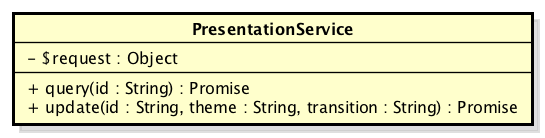
\includegraphics[width=0.4\linewidth]{img/premi_front_end_services_presentationservice}
		\caption[Premi::Front-End::Services::PresentationService]{Premi::Front-End::Services::PresentationService}
	\end{figure}
	
	\paragraph{Descrizione}
	Questa classe si occupa di gestire i processi di visualizzazione e modifica delle presentazioni.
	
	\paragraph{Utilizzo}
	Viene utilizzata per fornire ai controllers le funzionalità di interagire con le presentazioni nella fase di visualizzazione e modifica.
	
	\paragraph{Relazioni con le altre classi}
	\begin{itemize}
		\item \textbf{\textit{IN} ProjectController}
		Classe che gestisce le operazioni e la logica applicativa riguardante il progetto di un utente;
		\item \textbf{\textit{IN} PresentationController}
		Classe che gestisce le operazioni e la logica applicativa riguardante la visualizzazione di una presentazione;
		\item \textbf{\textit{IN} PresentationEditorController}
		Classe che gestisce le operazioni e la logica applicativa riguardante la modifica di una presentazione;
		\item \textbf{\textit{OUT} SlideEditorController}
		Classe che gestisce le operazioni e la logica applicativa riguardante la modifica delle slide.
	\end{itemize}
	
	\paragraph{Attributi}
	\begin{itemize}
		\item \textbf{+ \$http: Object}:\\
		Campo dati contenente un riferimento al servizio \textit{\$http} creato da Angular per facilitare la comunicazione tramite protocollo HTTP;
		\item \textbf{ProjectService: ProjectService};\\
		Campo dati per includere il service che gestisce i progetti.
	\end{itemize}
	
	\paragraph{Metodi}
	\begin{itemize}
		\item \textbf{+ loadPresentation(id)}:\\
		Metodo che richiede al back-end il caricamento della presentazione con id quello passato per parametro.
	\end{itemize}
	
	
\subsubsection{SlideService}
	\begin{figure}[h]
		\centering
		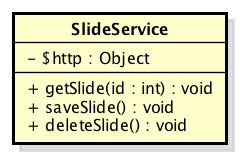
\includegraphics[width=0.4\linewidth]{img/premi_front_end_services_slideservice}
		\caption[Premi::Front-End::Services::SlideService]{Premi::Front-End::Services::SlideService}
	\end{figure}
	
	\paragraph{Descrizione}
	Questa classe si occupa di gestire i processi di modifica delle slide.
	
	\paragraph{Utilizzo}
	Viene utilizzata per fornire ai controllers le funzionalità di interagire con le slide nella fase modifica.
	
	\paragraph{Relazioni con le altre classi}
	\begin{itemize}
		\item \textbf{\textit{IN} PresentationEditorController}
		Classe che gestisce le operazioni e la logica applicativa riguardante la modifica di una presentazione;
		\item \textbf{\textit{OUT} SlideEditorController}
		Classe che gestisce le operazioni e la logica applicativa riguardante la modifica delle slide.
	\end{itemize}
	
	\paragraph{Attributi}
	\begin{itemize}
		\item \textbf{+ \$http: Object}:\\
		Campo dati contenente un riferimento al servizio \textit{\$http} creato da Angular per facilitare la comunicazione tramite protocollo HTTP.
	\end{itemize}

	\paragraph{Metodi}
	\begin{itemize}
		\item \textbf{+ getSlide(id)}:\\
		Metodo che richiede al back-end il caricamento della slide con id quello passato per parametro;
		\item \textbf{+ saveSlide()}:\\
		Metodo che richiede al back-end il salvataggio della slide corrente;
		\item \textbf{+ deleteSlide()}:\\
		Metodo che richiede al back-end la cancellazione della slide corrente e ritorna la slide successiva.
	\end{itemize}